% ****** Start of file aipsamp.tex ******
%
%   This file is part of the AIP files in the AIP distribution for REVTeX 4.
%   Version 4.1 of REVTeX, October 2009
%
%   Copyright (c) 2009 American Institute of Physics.
%
%   See the AIP README file for restrictions and more information.
%
% TeX'ing this file requires that you have AMS-LaTeX 2.0 installed
% as well as the rest of the prerequisites for REVTeX 4.1
%
% It also requires running BibTeX. The commands are as follows:
%
%  1)  latex  aipsamp
%  2)  bibtex aipsamp
%  3)  latex  aipsamp
%  4)  latex  aipsamp
%
% Use this file as a source of example code for your aip document.
% Use the file aiptemplate.tex as a template for your document.
\documentclass[%
 aip,
 % apl,
% jmp,%
% bmf,%
% sd,%
% rsi,%
 amsmath,amssymb,
% preprint,%
 reprint,%
% author-year,%
% author-numerical,%
 floatfix,%
]{revtex4-1}

\usepackage[utf8]{inputenc}
\usepackage{tikz}
\usepackage{graphicx}% Include figure files
\usepackage{dcolumn}% Align table columns on decimal point
\usepackage[T1]{fontenc}
\usepackage{bm}% bold math
\usepackage{mathptmx}
%\usepackage[mathlines]{lineno}% Enable numbering of text and display math
%\linenumbers\relax % Commence numbering lines
\usetikzlibrary{arrows,decorations.markings,decorations.pathmorphing, patterns,shapes}

\begin{document}

\preprint{AIP/123-QED}

\title[]{The Double Pendulum:\\Creating a Better Baseball Bat}
%\thanks{Footnote to title of article.}

\author{Jared Baur}
%\altaffiliation[Also at ]{Physics Department, Occidental College.}%Lines break automatically or can be forced with \\

\date{\today}% It is always \today, today,
             %  but any date may be explicitly specified

\begin{abstract}
	abstract goes here
\end{abstract}

\maketitle

% \onecolumngrid

\section{\label{sec:level1}Introduction}

The double pendulum is a classic example of chaotic motion\cite{Shinbrot1992}. The trajectories of various trials will show that the motion of a double pendulum is highly unpredictable. The chaos in a classic double pendulum is described by Equation 1. The exponent $\lambda$ is a positive constant, $\Delta x$ is the trajectory of the bottom arm of the pendulum, and $t$ is time. For small times $t$, the trajectories are relatively the same, however for increasing times, the trajectories exponentially increase in distance from trial to trial.
\begin{equation}
	\Delta x(t) \sim \Delta x(t_0) e^{\lambda t}
\end{equation}

\begin{figure}
	\centering
	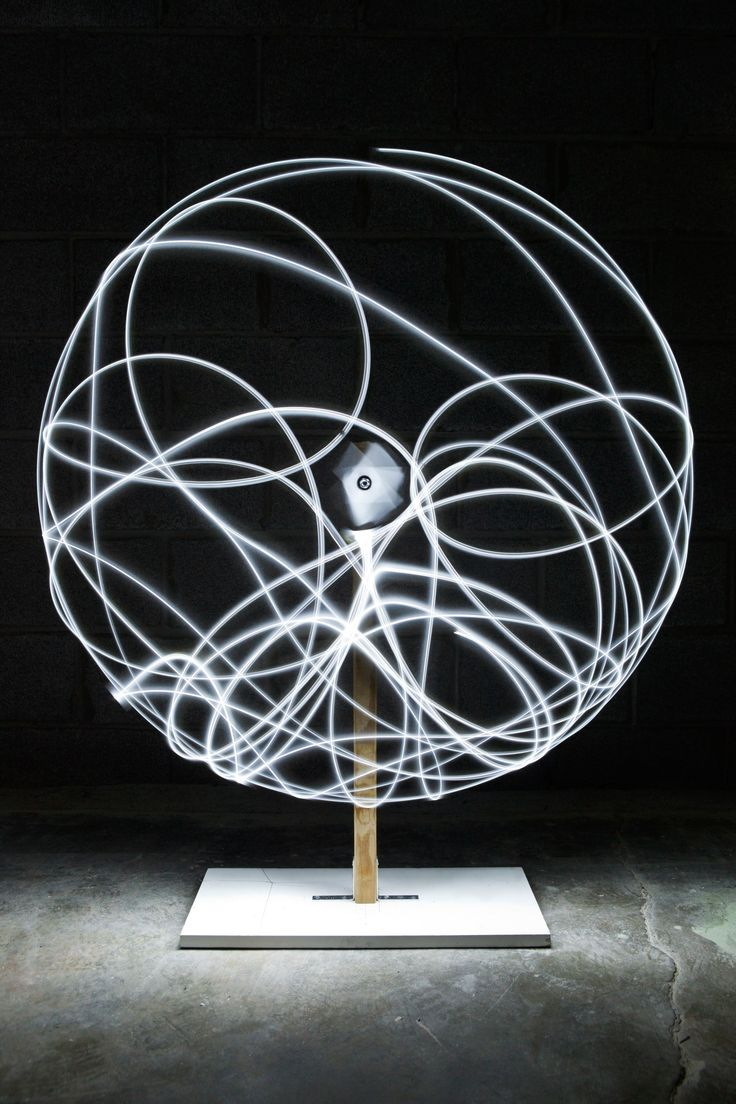
\includegraphics[scale=0.25]{lights.jpg}
	\caption{Chaos in a double pendulum. This figure depicts the trajectory of the end of the bottom arm in the double pendulum. The light is traced along the route of the bottom arm. As seen, there is no evident pattern in the bottom arm's trajectory.}
\end{figure}

The double pendulum is used in real life situations such as in double-trailer trucks (officially known as ``long combination vehicles") where two large-wheeled vehicles are combined at a hinge point. These vehicles are essentially semi-trucks with two trailers attached instead of one. The swinging motion in sports is also a common instance of a double pendulum. For this paper, the double pendulum will be compared to a baseball swing. In a baseball swing, a bat (striking implement) is used in conjunction with the arms to strike a baseball. In general, the arms are held up and back from the player's head, with the bat pointed upwards. The arms initiate the swing, moving towards the center of the player's body; the bat follows the arms, and then swings through as the transfer of energy from the arms to the bat occurs. This motion occurs mostly in the horizontal plane, but nonetheless acts as a double pendulum with the player's arms and the bat as the upper and lower ``arms" of the pendulum, respectively.

Since the swing of a baseball bat only occurs once per trial (does not swing back and forth and time $t$ is relatively low), this motion is equivalent to the first half cycle of a double pendulum swing. Thus, the chaotic motion prevalent in classic double pendulums will not be applicable for the purpose of the baseball swing.

Although the focus of this paper will be on the baseball swing, the double pendulum motion can be applied to the motion of a swing of a baseball bat, golf club, tennis racquet, or any other "swinging" motion that occurs with a striking implement. The goal of this paper will be to quantitatively describe the double pendulum in the context of a baseball swing and determine whether all of the energy in the striking implement can be transferred to the ball on impact. From this, we will decide whether we can design a baseball bat or ball that would allow for this perfect transfer of energy to occur.

\section{\label{sec:level2}Equations of Motion}

Describing the motion of a double pendulum has been argued as highly complicated\cite{Jorgensen1970}. For this reason, Lagrangians have been used in past studies to represent this motion. However, when we look at the forces on each arm of the pendulum with respect to each arm's center of mass, Newtonian equations of motion can be used to describe the motion.

Figure 2 depicts the components in a simple double pendulum. The upper arm of the pendulum is the first arm attached to a fixed axis $A$. This arm has length $L_1$, center of mass at point $G_1$, and distance to its center of mass $h_1$ (measured from point $A$). This arm makes an angle $\theta$ with the vertical axis and has a gravitational force acting on its center of mass equal to $M_1 g$, where $M_1$ is the mass of the arm and $g$ is the acceleration due to gravity.
\begin{figure}
	\centering
	\begin{tikzpicture}
		\node [inner sep=0pt,above right]
		{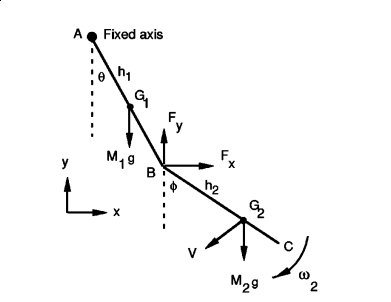
\includegraphics[scale=0.6]{equationsofmotion.png}};

		\draw[<->] (2,2.85) -- (0.5,5.5);
		\node (none) at (1,3.8) {$L_1$};

		\draw[<->] (5.5,2.85) -- (7.9,1.3);
		\node (none) at (6.9,2.4) {$L_2$};

	\end{tikzpicture}
	\caption{The components in a double pendulum. Since the equations that describe a double pendulum can be rather confusing, we use the center of mass $G_1$ and $G_2$ to describe the forces acting on the pendula arms.}
\end{figure}

		\begin{equation}
			L_1 \sin{\theta} + h_2 \sin{\phi} - L_1 \cos{\theta} - h_2 \cos{\phi}
		\end{equation}

		\begin{equation}
			V_x = \frac{dx}{dt} = -L_1 \omega_1 \cos{\theta} - h_2 \omega_2 \cos{\phi}
		\end{equation}
		\begin{equation}
			V_y = \frac{dy}{dt} = -L_1 \omega_1 \sin{\theta} - h_2 \omega_2 \sin{\phi}
		\end{equation}


		\begin{equation}
			\begin{aligned}
				F_x & = M_2 \frac{d V_x}{dt} \\
				    & = -M_2 \bigg [ L_1 \cos{\theta} \frac{d \omega_1}{dt} + L_1 \omega_1^2 \sin{\theta} \\
				    & + h_2 \cos{\phi} \frac{d \omega_2}{dt} + h_2 \omega_2^2 \sin{\phi} \bigg ]
			\end{aligned}
		\end{equation}

		\begin{equation}
			\begin{aligned}
				F_y - M_2 g & = M_2 \frac{d V_y}{dt}\\
				   & = -M_2 \bigg [ L_1 \sin{\theta} \frac{d \omega_1}{dt} - L_1 \omega_1^2 \cos{\theta} \\
				   & + h_2 \sin{\phi} \frac{d \omega_2}{dt} - h_2 \omega_2^2 \cos{\phi} \bigg ]
			\end{aligned}
		\end{equation}







\section{\label{sec:level3}Experimental Results}

\section{\label{sec:level4}Torque}

\section{\label{sec:level5}Energy Transfer}

\section{\label{sec:level6}Conclusion}

\nocite{*}
\bibliography{main.bib}% Produces the bibliography via BibTeX.

\end{document}
%
% ****** End of file aipsamp.tex ******
